\chapter{A cognitive approach to represent automotive scenes}%
\label{chap:a_cognitive_approach_to_represent_automotive_scenes}

We have seen in chapter ~\ref{chap:research_context}, especially in section ~\ref{subsec:knowledge_representation}, that, already today, there is a plethora of \acfp{ADAS} in intelligent vehicles. 
In future vehicles, the number of modules tackling different sub-tasks necessary to enable (semi-) autonomous driving and to interact with humans inside and outside the car will increase even more.
Given the complexity of the physical world and the recent success of \acp{DNN} in the diverse applications, a substantial amount of such modules could be data-driven with increasingly large neural networks under the surface.
In a worst case scenario, each of these systems will encapsulate its own representation of knowledge about the data it processes in complete separation from other, potentially related systems.
Typically, the representations used rely completely on numerical values and lack possibilities to be enriched or combined with symbol-like representations.
On the other hand, increasingly deep neural network architectures are not only hungry for data to generalize sufficiently enough from the examples they have been trained on, but also tend to require a substantial amount of computational resources.
Although this aspect is more severe for the training process, it becomes more important for mobile applications such as automated vehicles during the deployment phase.

In this thesis, we propose a novel representation for automotive scenes based on modern cognitive modeling techniques, namely the \ac{SPA}.
The \ac{SPA} is one particular example from a family of cognitive architectures commonly referred to as \acp{VSA} (see section ~\ref{subsec:vector_based_approaches} and chapter ~\ref{chap:introduction_to_vsas} for further details).
One of the key components of these cognitive architectures is to use high-dimensional vectors for representation.
This representational approach offers several desirable features.
High-dimensional vectors are one variant of distributed representations in the sense, that information is captured over all dimensions of the vector instead of one single number.
This aspect makes distributed representations more robust to noise in the sense, that a few noisy entries influence the overall information carried by the vector less compared to low-dimensional representations.
Furthermore, vector representations allow to encode both, symbol-like and numerical structures in a similar and unified way.
Additionally, the algebraic operations enable manipulation and combination of represented entities into structured representations.
One potential advantage of this approach is that the number of dimensions remains fixed independent of the number of entities combined through the architecture's algebraic operations.
Finally, vectors are a suitable representational substrate to be used in combination with neural networks.
On the one hand, vectors are a natural input to classic \acp{ANN}, but they also offer the possibility to be efficiently implement in \acp{SNN} using the principles of the \ac{NEF} (see \cite{Eliasmith2013}, but also section ~\ref{subsec:implementation_in_snns}).
Given an widespread implementation of the representations proposed here in combination with \acp{SNN} as algorithmic substrate within intelligent vehicles, the latter offers the potential to deploy such neural representations on dedicated neuromorphic hardware (cf.\ section ~\ref{sec:neuromorphic_HW}).
Although neuromorphic computing hardware as well as the corresponding neural algorithms are mainly used in academic research and often lack the technical maturity required by industrial applications, they show promise to be an energy-efficient option for future automated vehicles once reaching the required level of maturity.

\begin{figure}[t]
    \centering
    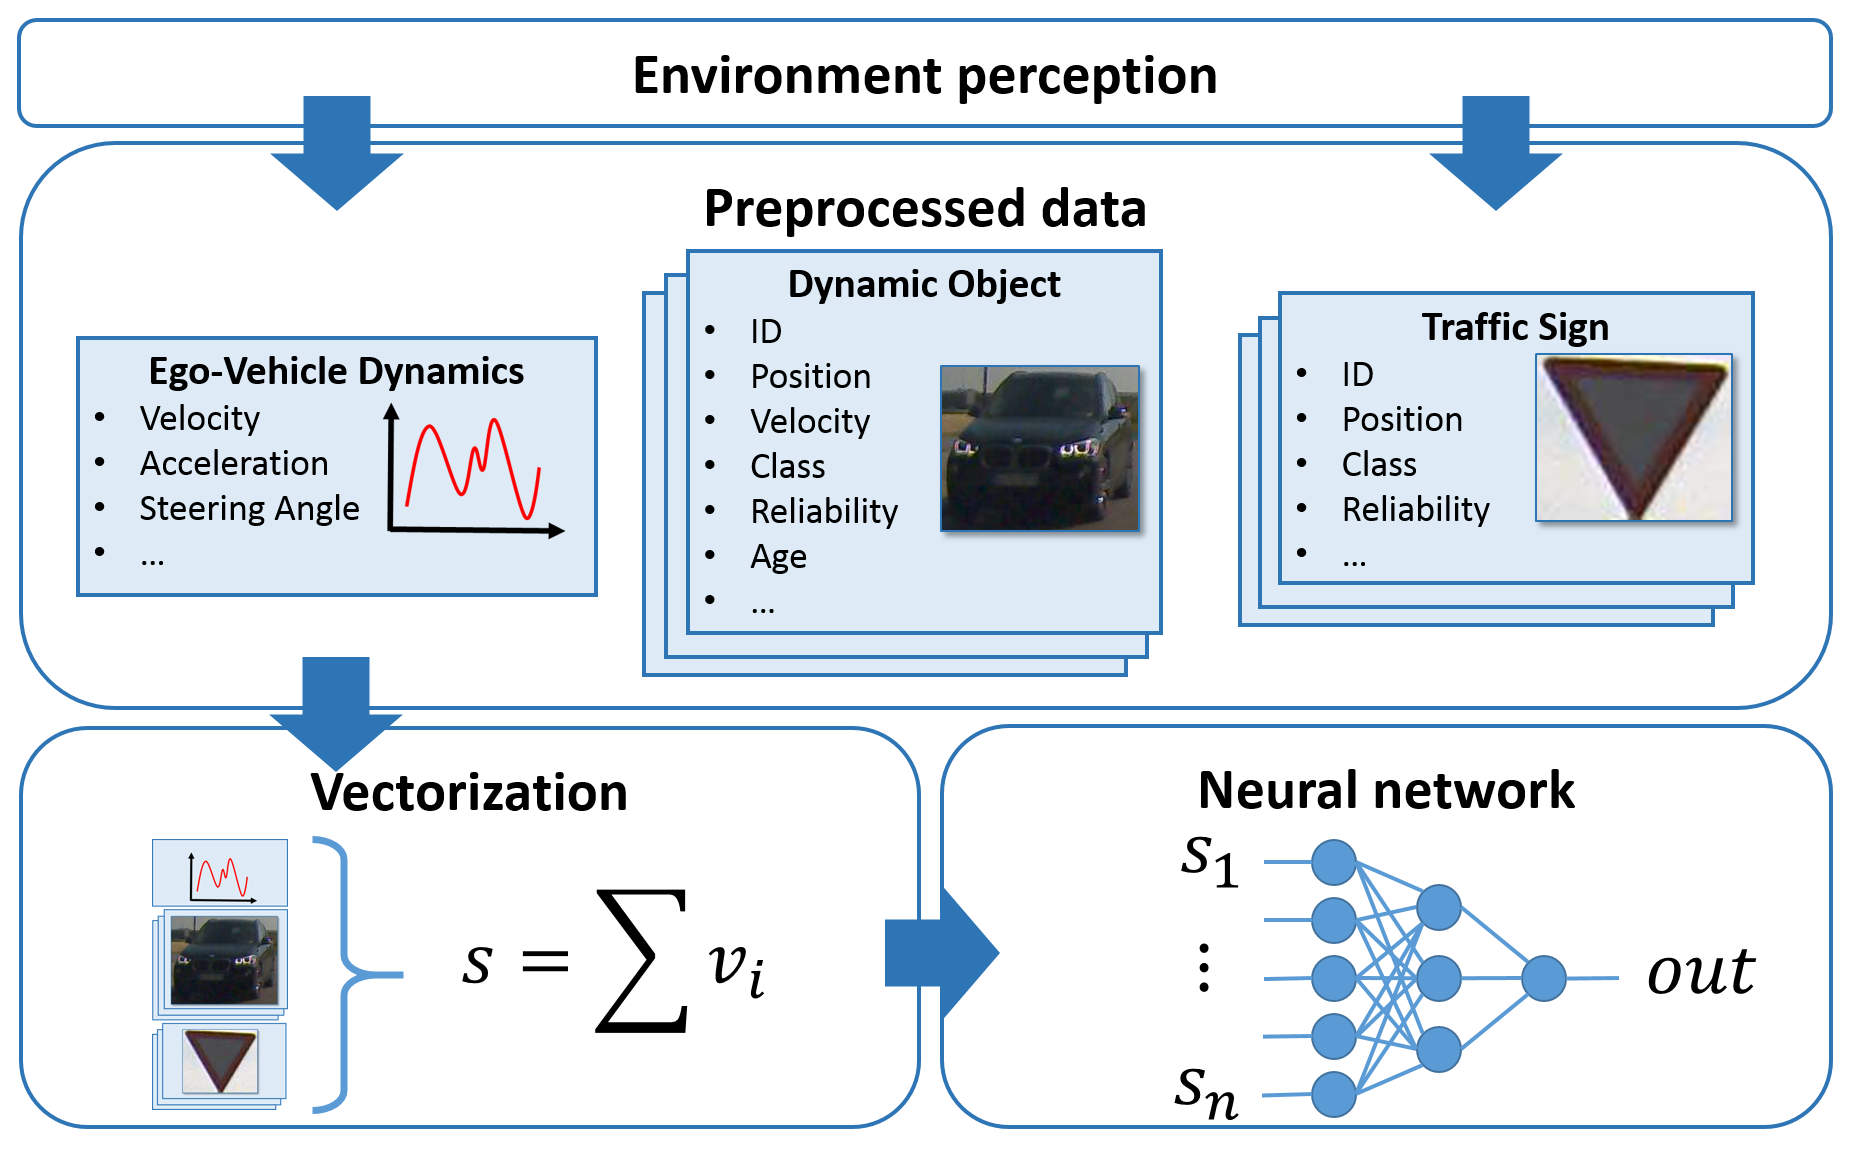
\includegraphics[width=0.8\linewidth]{imgs/system_overview_horizontal.eps}
    \caption{Visualization of the general flow of information of our proposed approach.}
    \label{fig:vectorization}
\end{figure}

In this chapter, we introduce our proposed approach to encapsulate high-level information about automotive scenes in high-dimensional, semantic vectors using the \ac{SPA} as representational substrate.
For this encoding phase, we follow the first two stages, namely \emph{preprocessing} and \emph{representation generation}, of the three-stages process established in \cite{Gallant2013} 
The third and final stage, \emph{output computation}, will be subject of subsequent chapters, where we investigate concrete applications and use cases.
The preprocessing stage is the step of creating a suitable vector vocabulary, whereas the representation generation stage is the process of building up structured representations from the atomic vectors within the vocabulary.
Furthermore, we analyze how different types of data could be encoded in such a representation, we show possible variations of how to encapsulate data in vectors and how they influence the final representation.
We also investigate potential limitations imposed bu such representations to provide insights into how many concepts can be efficiently encoded in our representations without loss of information.  


\section{Preprocessing stage - generating a vocabulary}%
\label{sec:preprocessing_stage_generating_a_vocabulary}

Fig. ~\ref{fig:vectorization} visualizes the general flow of information of our proposed system.
To represent high-level information about a scene in an abstract vector representation, we work with already processed data, which comes either from individual sensors, which perform their own low-level processing, or from a higher-level, central module already fusing information from several sensors.
We simply refer to this step as \emph{environment perception} in fig. ~\ref{fig:vectorization}, whereas its output is referred to as \emph{preprocessed data}.
This data is typically available as lists of objects present in the current scene and is translated into a semantic vector representation by first assigning atomic vectors to entities of interest and then building up more complex, structured representations by using the \ac{SPA}'s algebraic operations.
In this section, we will investigate the first step of assigning atomic vectors to entities of interest, i.e., creating a suitable vector vocabulary.
We have already seen in section ~\ref{subsec:vocabs}, that such vocabularies can be created in several different ways, which we will investigate with the specific focus of encoding automotive scenes.

\subsection{What types of data to encode?}%
\label{subsec:what_types_of_data_to_encode_}

The data to be encoded in a semantic vector substrate depends not only on the information available from the current sensor-setup, but also on the task at hand.
For instance, if we want to classify the current driving context (like in chapter ~\ref{chap:driving_context_classification}), the relevant information might be different to the task of predicting a vehicle's trajectory (like in chapter ~\ref{chap:behav_pred}).
Here, we give an overview of what information in general is available in an intelligent vehicle and how to encode it in a semantic vector substrate.
We distinguish between symbol-like information such as the type of a dynamic object or numerical information such as the current acceleration of the ego-vehicle.
In this section, we focus mainly on the symbol-like information, which is suitable to be represented using a single atomic vector or an algebraic combination of several atomic vectors.
In section ~\ref{subsec:different_vector_representations_for_numerical_values}, we will focus on numerical information and different options of encoding them in vectors,
Here, we will closely follow the structure of section ~\ref{sec:cognitive_modelling_with_vsa} and present different possibilities to generate a vocabulary of atomic vectors to built structured representations upon.

If the vectors in the vocabulary are not chosen at random, the general goal when creating the vocabulary is to generate atomic vectors that carry inherent structure or meaning.
This meaning is typically reflected by similar concepts being mapped to similar vectors.
However, there are several possible notions of similarity that can be encoded in the vocabulary, which we will specify in this section.

\subsubsection{Visual similarity}%
\label{ssubsec:visual_similarity}

A first simple and comprehensible notion of similarity is visual similarity between two entities: "do they look similar". 
Encoding this notion in vectors, we would expect the vector representations to represent this type of similarity within the relation between the vectors, meaning that vectors representing visually similar entities will have large cosine similarity.
In conjunction with other information, this type of similarity could be useful to detect a wrong classification, in case it has high similarity to another one that makes more sense in the situation or context at hand.
An example would the German traffic signs indicating a speed limit of \SI[per-mode=symbol]{30}{\kilo\meter\per\hour} and \SI[per-mode=symbol]{80}{\kilo\meter\per\hour}, which are both circular with a red frame and a similar looking black number on white background in the middle.
However, encountering a speed limit sign of \SI[per-mode=symbol]{30}{\kilo\meter\per\hour} in an urban situation is more plausible than a sign indicating a speed limit of \SI[per-mode=symbol]{80}{\kilo\meter\per\hour}.

\subsubsection{Similarity of motion}%
\label{ssubsec:similarity_of_motion}

Another notion of similarity, that is a candidate to be encoded in a vector vocabulary is the similarity of motion properties.
For instance, bicycles and motorcycles have more similar motion properties (dynamics of vehicles with two wheels) than for example a pedestrian and a truck.
Apart from motion properties such as dynamics of the movement, the number of wheels or the mean expected velocity the direction of movement of traffic participants can be a notion of similarity to be encoded in the vocabulary.
For instance, traffic participants such as bicycles or cars moving towards us might be encoded more similarly to each other than to parked cars or those moving away.
Furthermore, some entities are more likely to change their motion or direction: while traffic lights frequently alternate and parked cars might start moving, trees, buildings and traffic signs are expected to remain static. 
The notion of similarity of motion can be useful in various ways.
In a first step, knowing the motion of other traffic participants could help in classifying the situation: on a multi-lane highway we would expect cars around us to move in the same direction, whereas in an urban driving situation the motion of other traffic participants is more diverse. 
Additionally, this notion of similarity could potentially help in focusing the system's attention or more precisely, use computing power more efficiently on entities that are more relevant to decision making.
For example, a change of the 'motion status' (e.g.\ when a bus stops) might need particular attention.

\subsubsection{Semantic similarity}%
\label{ssubsec:semantic_similarity}

While visual similarity already captures a significant part of perceivable information about entities in automotive context, there is further information that could be encoded in the vector vocabulary that is different, and maybe even, contrary to visual similarity. 
Considering automotive situations, we as humans do not only assess them based on visual appearance but also by incorporating underlying and, most likely, previously acquired knowledge about the objects in the scene.
This underlying information can be considered the semantic aspect.
Revisiting the aforementioned example, the speed limit sign for \SI[per-mode=symbol]{30}{\kilo\meter\per\hour} is \emph{viusally} more similar to \SI[per-mode=symbol]{80}{\kilo\meter\per\hour} than to \SI[per-mode=symbol]{20}{\kilo\meter\per\hour}.
However, in the context (or semantics) of an automotive situation such as driving in an urban environment, speed limit signs for \num{20} and \SI[per-mode=symbol]{30}{\kilo\meter\per\hour} should be contextually or semantically more similar than signs for \num{30} and \SI[per-mode=symbol]{80}{\kilo\meter\per\hour}, as they are more likely to appear in similar contexts and both describe the traffic rule restricting driving to slow velocities.

Semantic similarity is not quite as intuitive as visual similarity. 
In general, we want to encode objects and concepts sharing similarity in \emph{meaning} in vectors with a high cosine similarity.
However, it is not intuitively clear what similar meaning actually refers to and how to properly define semantic similarity in an automotive context.
In the field of generating word embeddings for natural language processing, the typical assumption is that words that share similarity in meaning appear in close proximity with high probability within text corpora.
This assumption could be transferred to automotive context as well, for instance thinking of traffic signs indicating speed limits appearing in similar contexts or driving situations such as urban driving compared to higher speed limit signs.
However, on the one hand it is not clear how to transfer this approach to other object classes such as traffic participants whose appearance probability is less context dependent than for traffic signs. 
On the other hand the process of automatically training a system to learn this form of embedding is not clear as it would probably demand for another learning model to extract contextual information from the rich features of driving contexts.
Therefore, will now focus on the potential meaning of objects appearing in an automotive environment and how their semantic meaning could be embedded into a vector representation while leaving aside intangible concepts representing vehicle dynamics such as "velocity" or "acceleration".

\paragraph{Traffic signs}%
\label{par:traffic_signs}

Any traffic sign carries an explicit meaning defined in traffic law and anyone with a driver's license should know its meaning and be able to immediately explain it.
The meaning of a traffic sign is an instruction for the driver's behavior to, for instance, not surpass a certain velocity or to give way to other traffic participants. 
There are sub-groups of signs with similar meanings, such as signs indicating speed limits, prescribed direction or warnings for potentially dangerous road conditions or to pay increased attention.
Encoding the semantic structure of traffic signs in a vector vocabulary, we expect not only all traffic signs will be similar but also that all signs within a certain sub-group end up being more similar to one another compared to signs from other subgroups. 
For instance, signs indicating speed limits should be similar to one another, ideally with signs indicating lower velocities such as \SI[per-mode=symbol]{20}{\kilo\meter\per\hour} and \SI[per-mode=symbol]{30}{\kilo\meter\per\hour} should be more similar than \SI[per-mode=symbol]{30}{\kilo\meter\per\hour} and \SI[per-mode=symbol]{130}{\kilo\meter\per\hour}. 
Beside their explicit meaning, the number of traffic signs is finite and limited to a small number compared to the number of words in a typical human-level language vocabulary.
Therefore it is possible to manually engineer their semantic similarity, which makes it easier to impose our human understanding onto the structure, although the resulting vocabulary will most likely differ from the structure an unsupervised learning model would pick up from the data. 

\paragraph{Traffic participants}%
\label{par:traffic_participants}

While the meaning of traffic signs is clear and explicit, it is far more difficult to derive a meaning of a traffic participant such as a car or a pedestrian or a measure of similarity between them.
It is unclear if a truck is semantically more similar to a motorcycle or to a car without considering any contextual information while ignoring similarity of motion properties, which have already been discussed in section ~\ref{ssubsec:similarity_of_motion}.
However, if we do consider contextual information, we as humans decide intuitively if a truck and a motorcycle are more similar when compared to a pedestrian by e.g., considering their velocity of motion or their vulnerability.
We also know from experience that the meaning of a car approaching from the right potentially means that it has the right of way when we encounter a situation at a crossroads without traffic signs indicating other right of way rules. 
Hence, the situational context has a significant impact on comprehending the "meaning" of traffic participants, which in most cases directly results in appropriate driving actions to take such as decelerating or changing the lane.
However, such a situational understanding is impossible to derive without additional information such as position, velocity or direction of each traffic participant.
Consequently, it is impossible to encapsulate such semantic or contextual similarity in a vector vocabulary directly but rather encode another notion of similarity for atomic vectors of traffic participants and built situational similarity through structured representations using the \ac{VSA}'s algebraic operations.

\subsubsection{Summary on similarity}%
\label{ssubsec:summary_similarity}

All of the aforementioned notions cover a certain aspect of similarity.
Ideally, it is desirable for a vector vocabulary to encapsulate more than one notion of similarity comparable to a human understanding all these different aspects of similarity.
However, it is not clear if it is helpful or even possible, to encapsulate several notions of similarity into one coherent vector vocabulary or if it is more suitable to have separate vocabularies for each similarity of interest and combine them in structured representations using the \ac{VSA}'s algebraic operations as mentioned e.g., in \cite{Crawford2016}.
For the remainder of this section, we give an overview over different options of how to generate vector vocabularies encoding their own notion of similarity.

\subsection{Random and manually engineered vocabularies}%
\label{subsec:basic_random_vocabularies}

The simplest possible option to generate a vocabulary of atomic vectors is to sample them randomly, in case of continuous \acp{VSA} such as the \ac{SPA}, from the $D$-dimensional unit sphere \cite{Voelker2017}.
Naturally, randomly chosen atomic vectors do not carry semantic meaning or any intended notion of similarity.
However, given a sufficiently large dimension $D$ of the chosen \ac{VSA} and its theoretical properties (see chapter ~\ref{chap:introduction_to_vsas}), we can assume that randomly chosen vectors will be dissimilar enough to avoid accidentally mistaking them for one another.
Another advantage of this simple approach is that is comparatively easy to create a vocabulary avoiding any complex learning system to embed the concepts of interest in semantic vectors.
On the other hand, if specific applications demand for the vectors to actually carry semantic information meaning that similar concepts need to be mapped to similar vectors for the application to succeed, this simple approach can be extended by manually engineering a vocabulary reflecting the desired similarity structure.
This is typically achieved by randomly choosing a set of auxiliary vectors and building atomic vectors with the desired similarity from them through the \ac{VSA}'s algebraic operations (cf.\ section ~\ref{subsec:vocabs}).
However, this approach is only feasible and appropriate for rather small sized vocabularies as manually designing semantic vectors with certain similarity properties becomes intractable quickly with an increasing number of concepts to be embedded.
Furthermore, manually designing vocabularies involves design choices by human engineers, which is sensitive to potentially undesired biases in the similarity structure of the vectors.
For instance, the example vocabulary created in section ~\ref{subsec:vocabs} solely focused on the motion characteristics and typical actuators of different traffic participants.
However as mentioned before, there are many other possible similarity structures such as visual (or auditory), motion or semantic similarity, to be considered when designing the vocabulary.

\subsection{Visual vocabularies}%
\label{subsec:visual_vocabularies}

The next step to generate vocabularies with an inherent similarity structure is to encapsulate visual similarity in a vector embedding.
Visual similarity is an intuitive concept and we can make an educated guess that this notion of similarity could be beneficial for several tasks when encoded directly in the vector vocabulary. 
However, it is preferable to automatically learn to embed visual similarity in vectors instead of manually engineering the similarity between entities as this approach does not scale well for an increasing number of items to be encoded.
One option for such an automated learning system to generate a structured vocabulary encoding visual similarity is to adapt a \acf{DNN} for image classification.
Such a neural network can be thought of as an efficient image compression machine.
While earlier and intermediate layers learn sensibility to visual features such as edges and shapes, the information in the image is compressed into a single dimension, namely the label, at the final classification layer.
Considering the special case of a \acf{CNN}, one option would be to simply use the output of one of the later fully-connected layers and regard it as a vector as we expect the vectors of visually similar images to be similar regarding their cosine similarity.
Here, we focus our efforts of generating a visual vector vocabulary to items of interest to automated driving, namely the aforementioned categories of traffic signs and traffic participants.

\subsubsection{Traffic signs}%
\label{ssubsec:traffic_signs}

\begin{figure}[t]
    \centering
    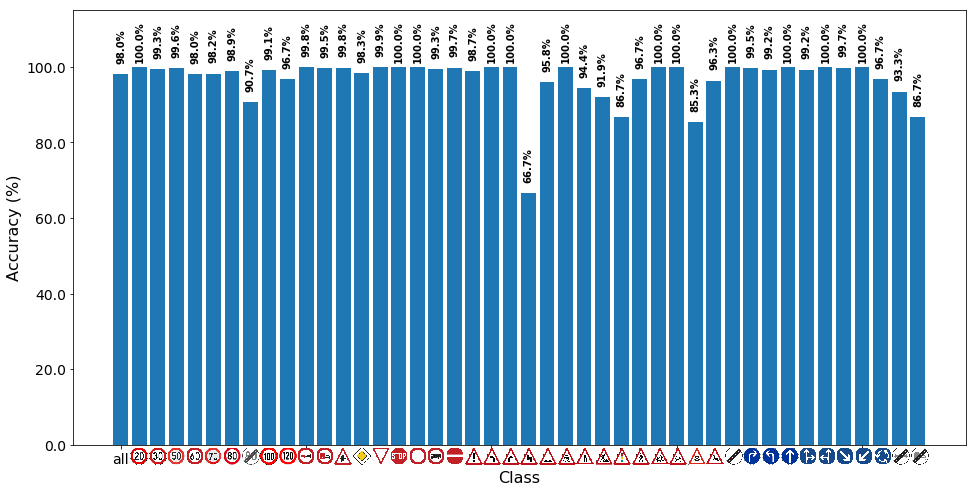
\includegraphics[width=0.9\linewidth]{imgs/CNN_GTSRB_performance_plot.png}
    \caption{Accuracy performance of the \ac{CNN} for traffic sign classification on the test part of the \ac{GTSRB} data set for all traffic signs (most left bar) and all individual traffic signs.}
    \label{fig:CNN_GTSRB_performance_plot}
\end{figure}

To achieve the task of encoding traffic signs encountered by an automated vehicle, we employ a variant of the state-of-the-art \ac{CNN} for traffic sign classification proposed in \cite{Ciresan2012}.
We train a simplified version of this network on the \acf{GTSRB} \cite{Stallkamp2012}, which is a data set including a total of \num{51840} images of \num{43} different classes of traffic signs.
Although the \ac{GTSRB} data set does not contain all possible traffic signs, it is a suitable and sufficiently large data set for our purposes of learning a visual vector vocabulary.
The original multi-column network proposed in \cite{Ciresan2012} combines several variants of the same network architecture trained on the original input images as well as four different, high-contrast normalized versions of the input images by averaging the predictions of all individual networks.
For simplicity, we only use a single-column version of this network to generate a visual vector vocabulary. 
Figure ~\ref{fig:CNN_GTSRB_performance_plot} shows the classification accuracy of our network on the test part of the \ac{GTSRB} data set for all traffic signs (most left bar) and all individual signs.
The network achieves competitive results with \SI{98}{\percent} classification accuracy on all traffic signs while detecting all but four traffic signs with accuracy values way above \SI{90}{\percent}, which is sufficient for our purposes.

\begin{figure}[t]
    \centering
    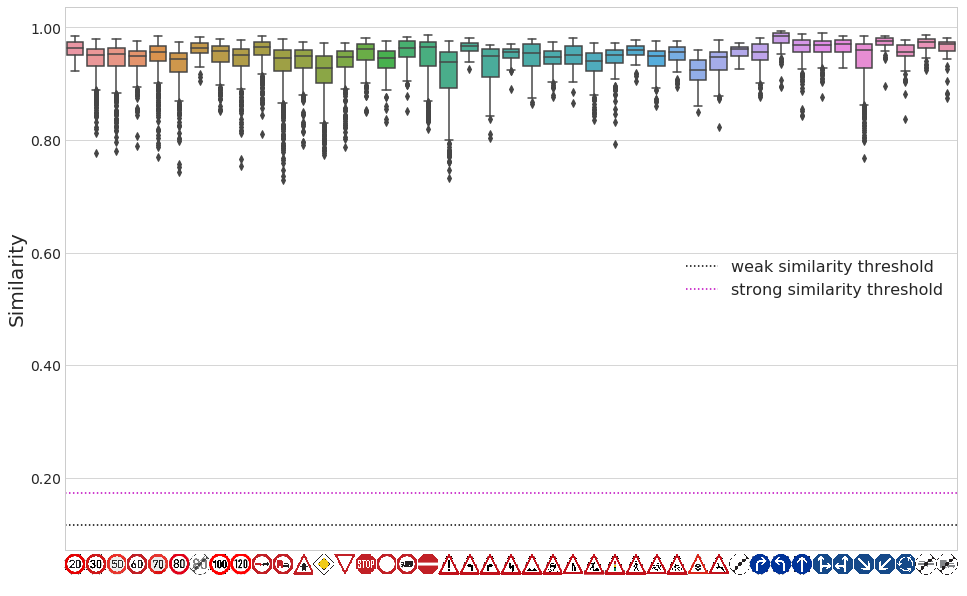
\includegraphics[width=0.9\linewidth]{imgs/Visual_vocab_traffic_signs_similarity_with_representative_vecs.png}
    \caption{Boxplots depicting the cosine similarities between the representative (mean) vector for each traffic sign class and all individual vector samples it has been created from.}
    \label{fig:visual_vocab_traffic_signs_similarity_with_representative_vecs}
\end{figure}

To generate our vocabulary vectors, we cut off the classification layer with softmax activation and use the previous \num{300}-dimensional, fully connected layer as output.
With this simple adaptation, the \ac{CNN} produces a \num{300}-dimensional vector as output for each image fed into the network. 
To generate a representative vector for each class of traffic signs, several approaches are conceivable, including (weighted) mean and median by dimension or regarding whole vectors.
In this work, we choose the simple mean to create this representative from several examples.
To select the example vectors to calculate the representative mean vector from, we select only instances for which the network produces correct classification predictions alongside high confidence values from the test subset of the \ac{GTSRB} data set.
The great majority of examples even satisfies the restriction of \SI{100}{\percent} confidence, hence we use that strict confidence value to avoid including examples the network is doubtful about, which might deteriorate the properties of the representative vector. 
This procedure leads to a representative vector that 'points' to the center of mass of all (high confidence) vectors of each class of traffic signs.
However, we still need to confirm that these representative vectors fulfill the properties they have been constructed for, namely sharing a high cosine similarity with all individual samples from the respective traffic sign class.
Fig. ~\ref{fig:visual_vocab_traffic_signs_similarity_with_representative_vecs} shows the cosine similarity between each vocabulary vector encoding each class of traffic signs with all individual vector samples it has been created from.
As expected, we observe high similarity values close to the maximum value of \num{1} and way above both, weak and strong, similarity thresholds for \num{300}-dimensional vectors.

\begin{figure}[t]
    \centering
    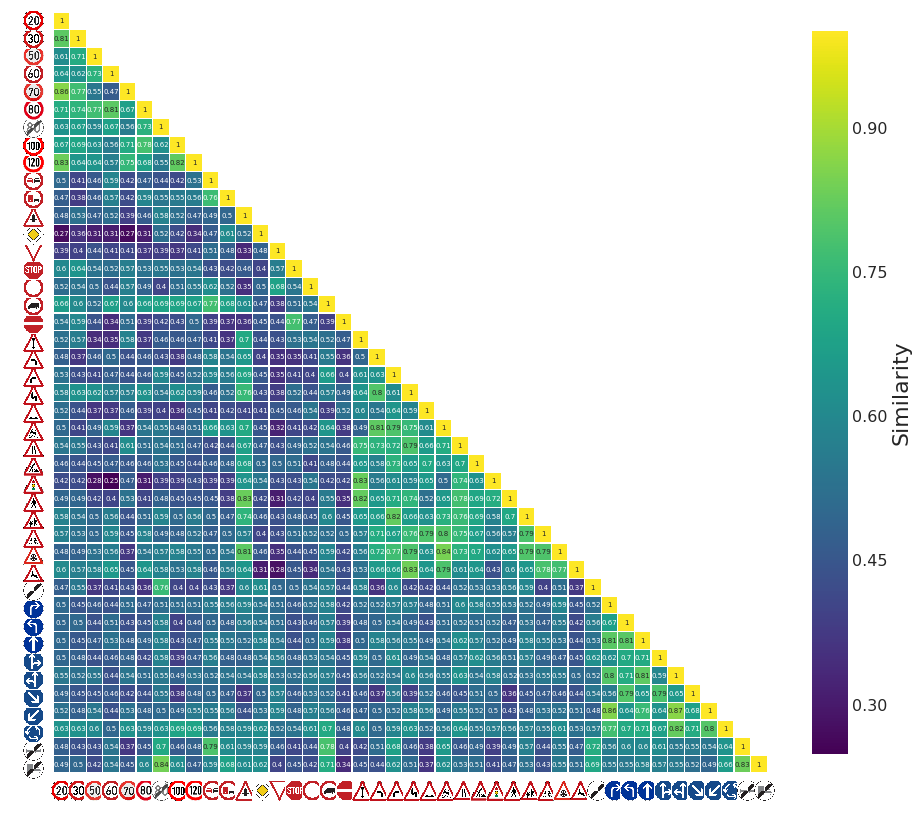
\includegraphics[width=0.8\linewidth]{imgs/visual_vocab_traffic_signs_internal_similarities.png}
    \caption{Pairwise similarities between representative vectors encoding traffic signs in a visual vector vocabulary.}
    \label{fig:visual_vocab_traffic_signs_internal_similarities}
\end{figure}

Furthermore, we expect these representative vectors, which are now our vocabulary vectors encoding the respective traffic signs, to resemble the visual similarity structure of the image classes. 
To confirm this inherent similarity structure, we calculate pairwise similarities between all vectors in the vocabulary, which are visualized in fig. ~\ref{fig:visual_vocab_traffic_signs_internal_similarities}.
We observe similarities in groups of signs indicated by green areas in the heat map visualization.
Most prominent are the high similarities in three groups of traffic signs forming green triangles in the heat map.
These groups are round signs with red borders (top left corner), triangular warning signs with red borders (middle right) and blue signs indicating driving directions (close to bottom right).
Furthermore, several signs stand out particularly: The traffic sign indicating "Priority ahead", which is a red triangle just like any warning signs, indeed shows high similarity to all warning signs.
Similarly, the traffic sign indicating no entry for trucks, a red circle with a black truck inside, looks a lot like speed limit signs and indeed shows a high similarity to all speed limit signs.
Consequently, we conclude that it is possible to encode visual similarity with an automatic learning approach using \acp{CNN} to encapsulate the visual features of a given data set into a vocabulary of semantic vectors.

\subsubsection{Traffic participants}%
\label{ssubsec:traffic_participants}
\begin{center}
	\begin{tabular}{|c|c|c|c|c|c|}
		\hline
		 & BICYCLE & CAR & MOTORCYCLE & PERSON & TRUCK\\ \hline
        Classification accuracy & \SI{94.3}{\percent} & \SI{76}{\percent} & \SI{55}{\percent} & \SI{82.6}{\percent}& \SI{99}{\percent}\\ \hline
	\end{tabular}
	\label{tab:traffic_participant_visual_accuracy}
	\captionof{table}{Classification accuracy of the adapted VGG19 network for our selected \num{5} classes of traffic participants.}
\end{center}

To encode the object categories for traffic participants \emph{Bicycle}, \emph{Car}, \emph{Motorcycle}, \emph{Pedestrian}, \emph{Truck} necessary to properly represent dynamic automotive scenes in visual vectors, we employ an approach similar to the one used for traffic signs.
We adopt a general purpose image data set, the Imagenet data set \cite{Deng2009}, which includes suitable categories for all of these classes.
As an additional advantage, Imagenet is a widely used data set, so there already exists a number of successful classification networks, which can be adapted for our purposes.
Concretely, we employ the following categories as they appear visually most suitable for the objects categories we want to encode:
We use the original labels 'SAFETY BICYCLE' to learn visual vectors for \emph{Bicycle}, 'USED CAR' for \emph{Car} (other car categories include ambulances and many sports / racing cars), 'MOTORCYCLE', 'PERSON' for \emph{Pedestrian} (since there is no special category for people in the vicinity of roads) and 'TRUCK'.
For each category, there are at least \num{1200} images available in the data set.

\begin{figure}[t]
    \centering
    \resizebox{.95\textwidth}{!}{%
        \subfloat[\label{subfig:visual_vocab_traffic_participants_similarity_with_representative_vecs}]{%
            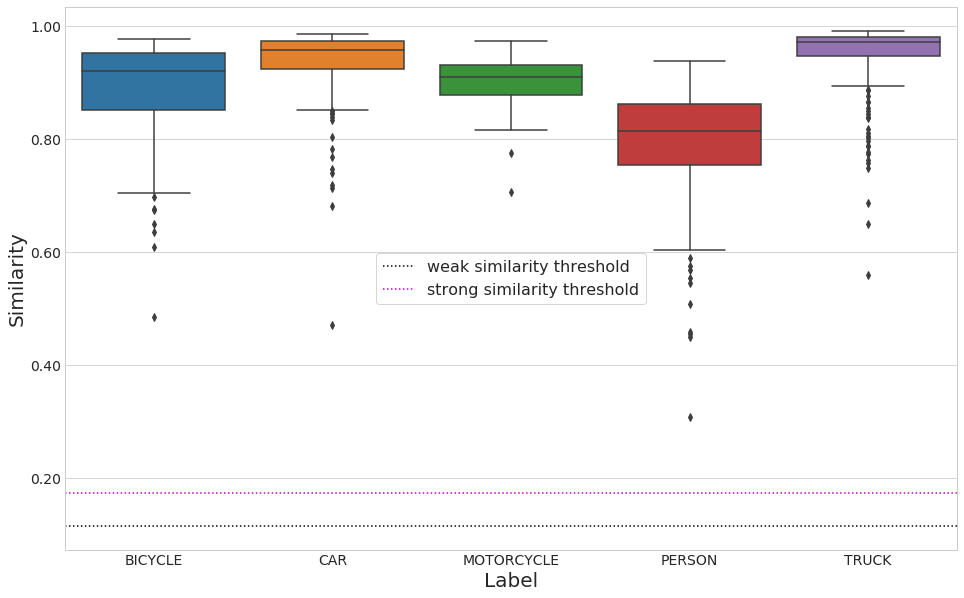
\includegraphics[height=3.5cm]{imgs/Visual_vocab_traffic_participants_similarity_with_representative_vecs.png}
        }
        \subfloat[\label{subfig:visual_vocab_traffic_participants_internal_similarities}]{%
            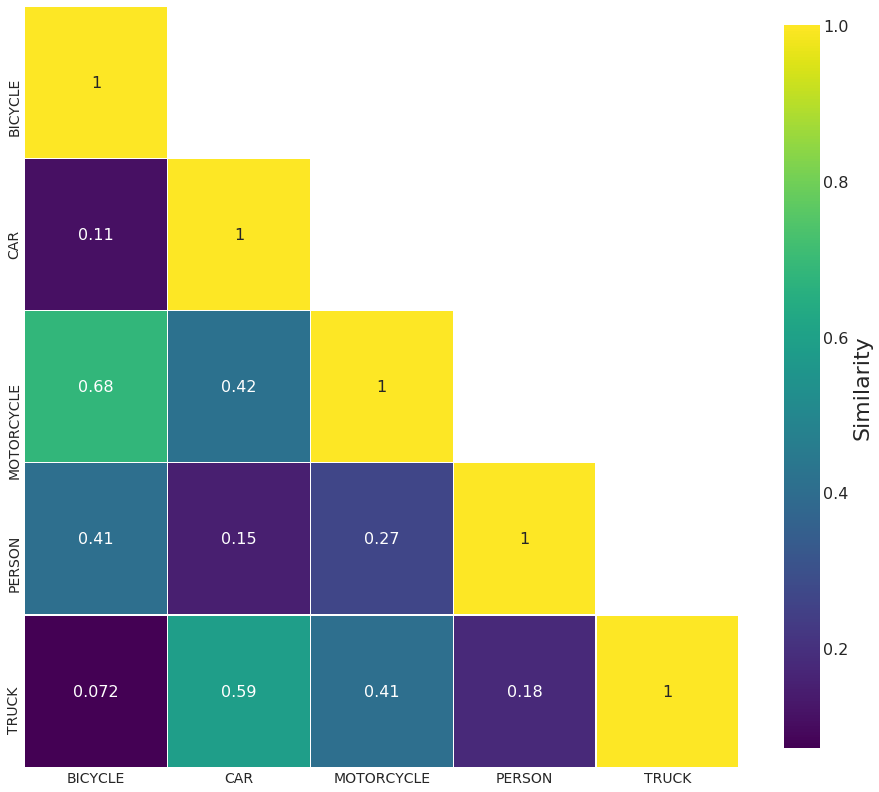
\includegraphics[height=3.5cm]{imgs/visual_vocab_traffic_participants_internal_similarities.png}
        }
    }
    \caption{Similarity plots for the visual vocabulary vectors representing traffic participants. ~\protect\subref{subfig:visual_vocab_traffic_participants_similarity_with_representative_vecs} Boxplots depicting the cosine similarities between the representative (mean) vector for each traffic participant class and all individual vector samples it has been created from. ~\protect\subref{subfig:visual_vocab_traffic_participants_internal_similarities} Pairwise similarities between representative
    vectors encoding traffic participants in our visual vector vocabulary.}
    \label{fig:visual_vocab_traffic_participants}
\end{figure}

While there is a number of state-of-the-art classification networks available achieving good results on the Imagenet data set, we are looking for a network with only moderately complex structure for the sake of implementation simplicity and ease of adaptation, while performance is of secondary priority.
VGG19 is a deep \acf{CNN} proposed in 2014 \cite{Simonyan2014} with a decent performance on the Imagenet data set (top 1 performance \SI{73}{\percent} and top 5 performance \SI{91}{\percent}) and a comparatively simple layer by layer architecture that allows easy extraction results from intermediate layers.
Our goal is to train a variant of the VGG19 network on these \num{5} classes and extract feature vectors of an intermediate layer to use them as vocabulary vectors.
Therefore, we adapt the original network architecture in the following way:
We cut off the last two fully connected layers as well as the classification layer and replace them with a fully connected, \num{300}-dimensional layer and a \num{5} dimensional classification layer. 
We train the modified network using the categorical cross entropy loss and 'standard' stochastic gradient descent optimization.

Table ~\ref{tab:traffic_participant_visual_accuracy} depicts the classification performance of our adapted VGG19 network for the \num{5} selected traffic participant categories.
Except for the 'MOTORCYCLE' class, the network achieves decent classification results above \SI{75}{\percent}, which is sufficient for our purposes.
Similar to the creation of the visual vocabulary for traffic signs, we calculate the of the network's correct predictions with \SI{100}{\percent} confidence.
Even for the 'MOTORCYCLE' class, there are at least \num{139} of such vectors available, whereas for all other classes, we have at least \num{200} of such vectors.
To confirm that the vocabulary vectors created in this fashion are visually representative enough for each class, we calculate the cosine similarity between the vocabulary vectors and all vector samples they have been created from.
Figure ~\ref{subfig:visual_vocab_traffic_participants_similarity_with_representative_vecs} visualizes these similarities as box plots.
Similar to the traffic sign vocabulary, we observe high similarity values close to the maximum value of \num{1} and way above both, weak and strong, similarity thresholds for \num{300}-dimensional vectors.
We also calculated pairwise similarities between all vocabulary vectors encoding traffic participants, which are visualized in figure ~\ref{subfig:visual_vocab_traffic_participants_internal_similarities}.
As expected, visually similar classes such as 'BICYCLE' and 'MOTORCYCLE' as well as 'CAR' and 'TRUCK' share relatively high cosine similarities.
Less similar, but still significantly higher than the similarity thresholds, are traffic participants sharing the visual features of persons such as 'PERSON' and 'BICYCLE', 'PERSON' and 'MOTORCYCLE' as well as 'BICYCLE' and 'MOTORCYCLE'.
All other pairs have similarity values in the order of magnitude or below the similarity thresholds and are therefore considered dissimilar while we do not attach the greatest importance to the actual (low) numbers.
Consequently, we can conclude, that we are able to encode visual similarity of traffic signs as well as traffic participants in a visual vector vocabulary.

\subsection{Semantic vocabularies}%
\label{subsec:semantic_vocabularies}

\begin{figure}[t]
    \centering
    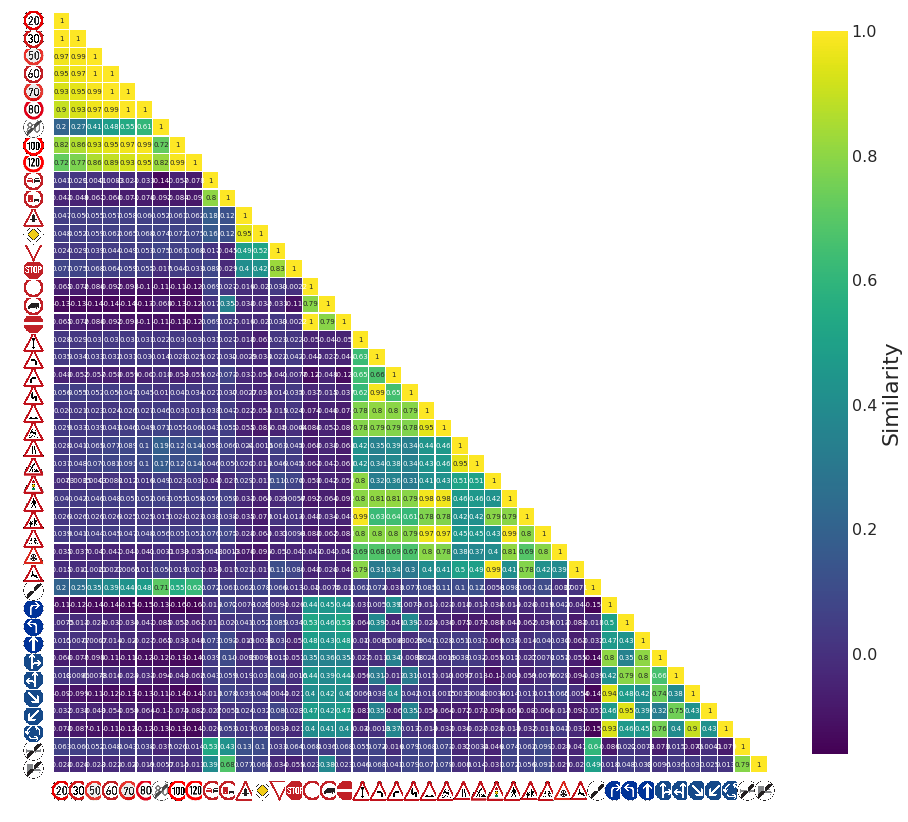
\includegraphics[width=0.8\linewidth]{imgs/semantic_vocab_traffic_signs_internal_similarities.png}
    \caption{Pairwise similarities between representative vectors encoding traffic signs in a manually designed semantic vector vocabulary.}
    \label{fig:semantic_vocab_traffic_signs_internal_similarities}
\end{figure}
In this section, we go one step further and try to encapsulate semantic similarity structures within a vector vocabulary.
As discussed in section ~\ref{ssubsec:semantic_similarity}, semantic similarity as a concept is comparatively intuitive for traffic signs and less obvious for other objects, such as traffic participants.
Furthermore, we also highlighted in that section that semantic similarity in other domains such as language modeling typically unfolds through proximity, i.e., that similar words appear in similar contexts or proximity within the text.
While this could give a hint towards what kind of learning procedure could be used to automatically generate a semantic vocabulary in automotive context, availability of suitable data sets is rather limited.
Analogously to the visual vocabulary, we consider the encoding of traffic signs and traffic participants separately in this section as well. 

\subsubsection{Traffic signs}%
\label{ssubsec:traffic_signs}

Our goal is to encode the meaning of traffic signs, i.e., the driving instruction or traffic rule they indicate to the driver in a semantic vector vocabulary.
As with visual similarity, this goal could be achieved by either manually engineering the similarity structure through the \ac{VSA}'s algebraic operations from randomly chosen atomic vectors or through some automated learning approach.
If we were to learn this automatically, there are two possible approaches. 
Similar to word embedding algorithms for language, we could either learn the meaning of traffic signs explicitly from a large  corpus of text that describes traffic signs and their meanings in context.
Alternatively, we could try to learn the semantic meaning of traffic signs implicitly from many dynamic driving situations.
Unfortunately, there are no suitable data sets available for either of the aforementioned learning approaches.
Additionally, an implementation of the latter, implicit learning approach would be quite complex, as it would require additional steps to extract structural understanding from the driving scene upon on which the vocabulary generation system needs to be built.
To our our knowledge, such a system does not exist.
Consequently, the only remaining option is to manually design the desired similarity structure as described in section ~\ref{subsec:basic_random_vocabularies}.

To encode the semantic meaning of traffic signs, we choose atomic vectors for the basic building blocks of the representation at random and create semantic structure by employing the algebraic operations of the \ac{SPA}.
We apply the role-filler pair approach described in section ~\ref{subsec:encoding_struct}.
We randomly choose vectors for the roles \textbf{TYPE} and \textbf{MEANING} encoding the type and the meaning of a particular traffic sign.
For some traffic signs, we need an additional role \textbf{REASON} giving further information to the vocabulary vector in order to distinguish similar traffic signs from one another.
As potential filler vectors for the \textbf{TYPE} role, we choose random vectors representing the following traffic sign classes included in the \ac{GTSRB}: \textbf{LIMIT}, \textbf{PASSING}, \textbf{PRIORITY}, \textbf{DIRECTION} and \textbf{ATTENTION}.
Similarly, we create filler vectors for the \textbf{MEANING} role like \textbf{RIGHTOFWAY}, \textbf{GIVEWAY}, \textbf{SLOW}, \textbf{PREPARETOSTOP}, \textbf{CONCENTRATE}, \textbf{LEFT}, \textbf{RIGHT}, \textbf{STRAIGHT}, \textbf{OVERTAKING}.
Finally, we create filler vectors for the \textbf{REASON} role indicating the reason for increased attention or other additional information such as \textbf{PEDESTRIANS}, \textbf{CHILDREN} or \textbf{SLIPPERYROAD}, \textbf{ROADWORKS} etc.
Given these role and filler vectors, we generate semantic vocabulary vectors encoding the meaning of traffic signs in the following way

\begin{equation}
    \label{eq:semantic_vocab_traffic_signs}
    \mathbf{SIGN} = \mathbf{TYPE} \varoast \mathbf{FT} + \mathbf{MEANING} \varoast \left( \sum\limits_{i=0}^{n} \beta_{i} \cdot  \mathbf{FM}_{i}  \right) + \gamma \cdot \mathbf{REASON} \varoast \mathbf{FR}, 
\end{equation}

where \textbf{FT}, $\mathbf{FM}_{i}$ for $i = 0, \ldots, n$ and \textbf{FR} are placeholders for the filler vectors and $\beta_{i} \in \mathbb{R} $ for $i = 0, \ldots, n$ and $\gamma \in \mathbb{R} $ are weighting factors.
In case, the additional \textbf{REASON} role is not needed for a particular traffic sign, the corresponding weight factor $\gamma$ is set to \num{0}.
For instance, the vocabulary vector encoding the traffic sign indicating danger is calculated as

\begin{equation}
\label{eq:semantic_vocab_traffic_sign_example}
\mathbf{DANGER} = \mathbf{TYPE} \varoast \mathbf{ATTENTION} + \mathbf{MEANING} \varoast  \left(\mathbf{SLOW} + \mathbf{PREPARETOSTOP}\right).
\end{equation}

Traffic signs indicating speed limits form somewhat of a special case, as we want to encode them in such a way, that signs indicting lower speed limits are more similar to one another than to signs indicating higher speed limits.
To achieve that, we need to encode numerical values that are closer to one another more similar than numerical values with larger intervals.
Here, we employ a very simple encoding scheme using the function 
\begin{equation}
\label{eq:cosin_vec_func}
\abb{\varphi}{i\mathbb{R}}{\mathbb{R}^{D}}{x}{\left(\sin(x), \cos(x), 0, \ldots, 0\right)}.
\end{equation}
In other words, we create a speed vector by setting the first two dimensions to $\sin(x)$ and $\cos(x)$ for the encoded numerical value $x \in [0,\frac{\pi}{2}]$ and all other entries to \num{0} (note that we will discuss other, more complex approaches to encode numerical values in vectors in section ~\ref{subsec:different_vector_representations_for_numerical_values}).
We use \SI[per-mode=symbol]{200}{\kilo\meter\per\hour} as general speed limit, i.e., we map all speed limit values between \num{0} and \num{200} to the interval $\left[0, \frac{\pi}{2}\right]$ with \SI[per-mode=symbol]{200}{\kilo\meter\per\hour} $\equiv \frac{\pi}{2}$.

Figure ~\ref{fig:semantic_vocab_traffic_signs_internal_similarities} shows the pairwise similarities between the manually designed semantic vectors encoding traffic signs in the \ac{GTSRB} created in the aforementioned fashion.
As expected, we see a highly structured area in the top left corner, the speed limit signs.
The other groups of signs (overtaking, priority, warning and direction) are also visible as triangles on the right hand side.
All non-related entities have low similarities of less than \num{0.1}.
Brighter spots in the large dark area to the left represent similarities across sign groups, especially, for signs related to trucks and curves or bends.
Consequently, we were successful in manually designing a vocabulary encapsulating semantic similarity of traffic signs as an alternative to the visual vocabulary created in section ~\ref{subsec:visual_vocabularies}.

\subsubsection{Traffic participants}%
\label{ssubsec:traffic_participants}

\begin{figure}[t]
    \centering
    \resizebox{.9\textwidth}{!}{%
        \subfloat[\label{subfig:semantic_vocab_traffic_participants_word2vec_internal_similarities}]{%
            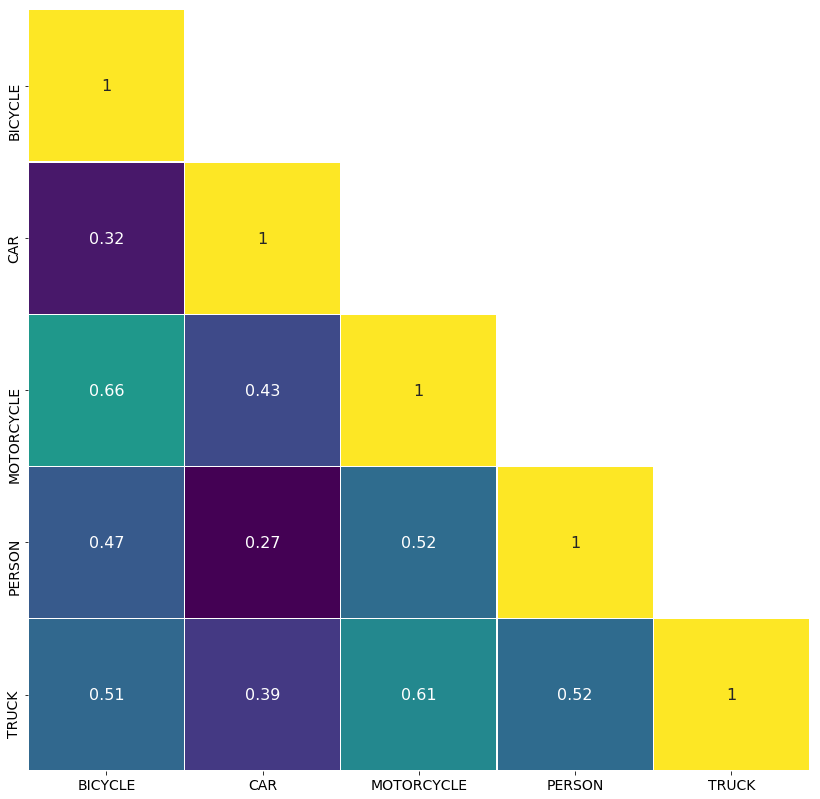
\includegraphics[height=3cm]{imgs/semantic_vocab_traffic_participants_word2vec_internal_similarities.png}
        }
        \subfloat[\label{subfig:semantic_vocab_traffic_participants_manual_internal_similarities}]{%
            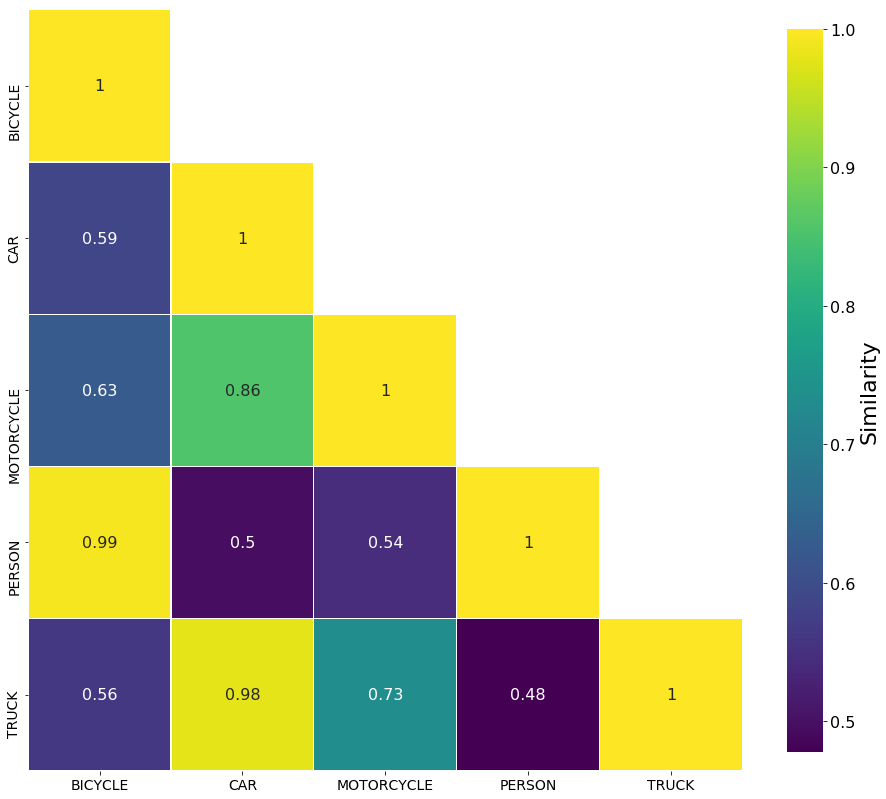
\includegraphics[height=3cm]{imgs/semantic_vocab_traffic_participants_manual_internal_similarities.png}
        }
    }
    \caption{Pairwise similarities between representative vectors encoding traffic participants in a semantic vector vocabulary. ~\protect\subref{subfig:semantic_vocab_traffic_participants_word2vec_internal_similarities} Learned with word2vec ~\protect\subref{subfig:semantic_vocab_traffic_participants_manual_internal_similarities} manually designed.}
    \label{fig:semantic_vocab_traffic_participants_internal_similarities}
\end{figure}

As discussed in section ~\ref{subsec:what_types_of_data_to_encode_}, semantic similarity for traffic participants is hard to capture intuitively.
We concluded that the general meaning of traffic participants is highly context-dependent, which in turn can only be learned from dynamic driving data of from a text corpus describing traffic situations.
However, such data sets are either not available or do not even exist.
Hence, as a first step towards the goal of encoding semantic similarity, we will therefore encapsulate the similarity between the five classes of traffic participants already discussed in section ~\ref{subsec:visual_vocabularies}, namely \emph{Bicycle}, \emph{Car}, \emph{Motorcycle}, \emph{Pedestrian}, \emph{Truck}.
Here, we employ two different approaches: an automated learning approach making use of the well-established word embedding of the word2vec algorithm \cite{Mikolov2013} trained on the Google News data set and, similar to the semantic vocabulary of traffic signs, manual design, which is only possible due to the small size of our vocabulary.
Word2vec is an unsupervised learning approach generating a word embedding, i.e., vectors representing every word encountered in the training text, where words that appear in similar context (close proximity within the text) are mapped to similar vectors. 
For our purposes, we simply extract the (\num{300}-dimensional) vectors representing the objects of interest (traffic participants) from the learned vocabulary.
The manually designed semantic vocabulary is generated similarly to the aforementioned vocabulary of traffic signs using the \ac{SPA}'s algebraic operation and the role-filler-pairs approach based on two key properties, which give good yet simple description of the traffic participant's semantic properties: speed and vulnerability represented by randomly chosen atomic vectors \textbf{SPEED} and \textbf{VULNERABILITY}.
Hence, we encode the five classes of traffic participants through

\begin{equation}
\label{eq:semantic_vocab_traffic_participants}
\mathbf{PARTICIPANT} = \mathbf{SPEED} \varoast \varphi(s) + \mathbf{VULNERABILITY} \varoast \varphi(v),
\end{equation}

using the encoding function $\varphi$ from equation ~\ref{eq:cosin_vec_func}.

Figure ~\ref{fig:semantic_vocab_traffic_participants_internal_similarities} depicts the pairwise similarities of both, the semantic vocabulary using word2vec vectors (figure ~\ref{subfig:semantic_vocab_traffic_participants_word2vec_internal_similarities}) and the manually designed vocabulary vectors (figure ~\ref{subfig:semantic_vocab_traffic_participants_manual_internal_similarities}.
We observe that the pre-trained word vectors from word2vec are not entirely successful to capture the kind of semantic similarity we are interested in.
While vectors are similar to each other, the individual similarities do not always match our human understanding, especially when considering an automotive context.
For instance, the vector encoding \emph{person} is significantly more similar to the one representing \emph{truck} than to the one representing \emph{car} while \emph{car} is the traffic participant least similar to \emph{truck}. 

For the manually designed vocabulary (figure \ref{subfig:semantic_vocab_traffic_participants_manual_internal_similarities}), results are more convincing.
We are able to achieve a higher similarity between vectors encoding \emph{car} and \emph{truck} as well as \emph{bicycle} and \emph{person} with lower similarities between \emph{person} and \emph{truck} as well as \emph{bicycle} and \emph{truck}.
This vocabulary is also not an ideal representation but gets much closer to the desired semantic structure between these entities in an automotive context. 

\subsection{Visual-semantic vocabularies}%
\label{subsec:visual_semantic_vocabularies}

results from Roberts thesis

\section{Representation generation stage}%
\label{sec:representation_generation_stage}


\subsection{Different vector representations for numerical values}%
\label{subsec:different_vector_representations_for_numerical_values}


In this section, we investigate different approaches to map numerical information to semantic vectors.
Therefore, we will focus on
problem of how to encode numerical information (vector length vs trigonomical vs. unitary vector powers) for values of position, velocity etc.
\subsubsection{Scalar multiplication encoding}
\subsubsection{Sine and Cosine encoding with different frequencies and offsets}
For vectorization of two-dimensional values, we use an encoding with sine and cosine functions with different spatial frequencies and offsets.
Therefore, we define the following helper functions
\[ \abb{f_{\left(m,i\right)}}{\mathbb{R}^2}{\mathbb{R}^4}{\left(x,y\right)}{\left(\cos\frac{m\cdot \pi + x}{i + 1}, \sin\frac{m\cdot \pi + x}{i + 1}, \cos\frac{m\cdot \pi + y}{i + 1}, \sin\frac{m\cdot \pi + y}{i + 1}\right)},
\]
\[
\abb{\psi_i}{\mathbb{R}^2}{\mathbb{R}^4}{\left(x,y\right)}{\left(f_{\left(0,i\right)}\left(x,y\right), f_{\left(\frac{1}{2},i\right)}\left(x,y\right), f_{\left(1,i\right)}\left(x,y\right), f_{\left(\frac{3}{2},i\right)}\left(x,y\right)\right)}
\]
and obtain the final vector representation of acceleration in $x$/$y$-direction via the function
\[
\abb{\lambda}{\mathbb{R}^2}{\mathbb{R}^D}{\left(x,y\right)}{\frac{1}{\sqrt{\frac{D}{2}}}\left(\psi_0\left(x,y\right), \cdots, \psi_{\frac{D}{16}-1}\left(x,y\right)\right).}
\]
This encoding $\lambda\left(a_x, a_y\right)$ leads to normalized, nonzero, similar vectors with information distributed over all elements (in contrast to a simple encoding like $\left(a_x, a_y, 0 \cdots, 0\right)$).
\subsubsection{Convolutive power encoding}

\subsection{Structured representations}%
\label{subsec:structured_representations}

\section{Capacity analysis - limitations to vector representations}%
\label{sec:capacity_analysis_limitations_to_vector_representations}

\subsection{Limiting factors to structured representations}%
\label{subsec:limiting_factors_to_structured_representations}


\begin{figure}[t]
	\centering
	\includegraphics[width=0.95\textwidth]{imgs/spa_superposition_capacity_1.png}
	\caption{Superposition capacity.}
	\label{fig:spa_superposition_capacity}
\end{figure}

\section{Summary}%
\label{sec:vector_representations_automotive_summary}
\todo[inline]{somewhere (maybe in one of the subsequent chapters) where it is fitting the option to adjust the vector embedding based on the performance on a certain task to potentially improve the model's task performance by a better vector embedding (something more of future work thing, not intended to be investigated in this thesis, but still worth mentioning)}


